% \documentclass[11pt,compress,t,notes=noshow, xcolor=table]{beamer}
% \usepackage[]{graphicx}\usepackage[]{color}
% % maxwidth is the original width if it is less than linewidth
% % otherwise use linewidth (to make sure the graphics do not exceed the margin)
% \makeatletter
% \def\maxwidth{ %
% 	\ifdim\Gin@nat@width>\linewidth
% 	\linewidth
% 	\else
% 	\Gin@nat@width
% 	\fi
% }
% \makeatother

% \definecolor{fgcolor}{rgb}{0.345, 0.345, 0.345}
% \newcommand{\hlnum}[1]{\textcolor[rgb]{0.686,0.059,0.569}{#1}}%
% \newcommand{\hlstr}[1]{\textcolor[rgb]{0.192,0.494,0.8}{#1}}%
% \newcommand{\hlcom}[1]{\textcolor[rgb]{0.678,0.584,0.686}{\textit{#1}}}%
% \newcommand{\hlopt}[1]{\textcolor[rgb]{0,0,0}{#1}}%
% \newcommand{\hlstd}[1]{\textcolor[rgb]{0.345,0.345,0.345}{#1}}%
% \newcommand{\hlkwa}[1]{\textcolor[rgb]{0.161,0.373,0.58}{\textbf{#1}}}%
% \newcommand{\hlkwb}[1]{\textcolor[rgb]{0.69,0.353,0.396}{#1}}%
% \newcommand{\hlkwc}[1]{\textcolor[rgb]{0.333,0.667,0.333}{#1}}%
% \newcommand{\hlkwd}[1]{\textcolor[rgb]{0.737,0.353,0.396}{\textbf{#1}}}%
% \let\hlipl\hlkwb

% \usepackage{framed}
% \makeatletter
% \newenvironment{kframe}{%
% 	\def\at@end@of@kframe{}%
% 	\ifinner\ifhmode%
% 	\def\at@end@of@kframe{\end{minipage}}%
% \begin{minipage}{\columnwidth}%
% 	\fi\fi%
% 	\def\FrameCommand##1{\hskip\@totalleftmargin \hskip-\fboxsep
% 		\colorbox{shadecolor}{##1}\hskip-\fboxsep
% 		% There is no \\@totalrightmargin, so:
% 		\hskip-\linewidth \hskip-\@totalleftmargin \hskip\columnwidth}%
% 	\MakeFramed {\advance\hsize-\width
% 		\@totalleftmargin\z@ \linewidth\hsize
% 		\@setminipage}}%
% {\par\unskip\endMakeFramed%
% 	\at@end@of@kframe}
% \makeatother

% \definecolor{shadecolor}{rgb}{.97, .97, .97}
% \definecolor{messagecolor}{rgb}{0, 0, 0}
% \definecolor{warningcolor}{rgb}{1, 0, 1}
% \definecolor{errorcolor}{rgb}{1, 0, 0}
% \newenvironment{knitrout}{}{} % an empty environment to be redefined in TeX

% \usepackage{alltt}
% \newcommand{\SweaveOpts}[1]{}  % do not interfere with LaTeX
% \newcommand{\SweaveInput}[1]{} % because they are not real TeX commands
% \newcommand{\Sexpr}[1]{}       % will only be parsed by R

% \usepackage[english]{babel}
% \usepackage[utf8]{inputenc}

% \usepackage{dsfont}
% \usepackage{verbatim}
% \usepackage{amsmath}
% \usepackage{amsfonts}
% \usepackage{bm}
% \usepackage{csquotes}
% \usepackage{multirow}
% \usepackage{longtable}
% \usepackage{booktabs}
% \usepackage{enumerate}
% \usepackage[absolute,overlay]{textpos}
% \usepackage{psfrag}
% \usepackage{algorithm}
% \usepackage{algpseudocode}
% \usepackage{eqnarray}
% \usepackage{arydshln}
% \usepackage{tabularx}
% \usepackage{placeins}
% \usepackage{tikz}
% \usepackage{setspace}
% \usepackage{colortbl}
% \usepackage{mathtools}
% \usepackage{wrapfig}
% \usepackage{bm}
% \usepackage[backend=biber]{biblatex}

% \usetikzlibrary{shapes,arrows,automata,positioning,calc,chains,trees, shadows}
% \tikzset{
% 	%Define standard arrow tip
% 	>=stealth',
% 	%Define style for boxes
% 	punkt/.style={
% 		rectangle,
% 		rounded corners,
% 		draw=black, very thick,
% 		text width=6.5em,
% 		minimum height=2em,
% 		text centered},
% 	% Define arrow style
% 	pil/.style={
% 		->,
% 		thick,
% 		shorten <=2pt,
% 		shorten >=2pt,}
% }

% \usepackage{subfig}

% % Defines macros and environments
% % This file is included in slides and exercises

% Rarely used fontstyle for R packages, used only in 
% - forests/slides-forests-benchmark.tex
% - exercises/single-exercises/methods_l_1.Rnw
% - slides/cart/attic/slides_extra_trees.Rnw
\newcommand{\pkg}[1]{{\fontseries{b}\selectfont #1}}

% Spacing helpers, used often (mostly in exercises for \dlz)
\newcommand{\lz}{\vspace{0.5cm}} % vertical space (used often in slides)
\newcommand{\dlz}{\vspace{1cm}}  % double vertical space (used often in exercises, never in slides)
\newcommand{\oneliner}[1] % Oneliner for important statements, used e.g. in iml, algods
{\begin{block}{}\begin{center}\begin{Large}#1\end{Large}\end{center}\end{block}}

% Don't know if this is used or needed, remove?
% textcolor that works in mathmode
% https://tex.stackexchange.com/a/261480
% Used e.g. in forests/slides-forests-bagging.tex
% [...] \textcolor{blue}{\tfrac{1}{M}\sum^M_{m} [...]
% \makeatletter
% \renewcommand*{\@textcolor}[3]{%
%   \protect\leavevmode
%   \begingroup
%     \color#1{#2}#3%
%   \endgroup
% }
% \makeatother


% %\usetheme{lmu-lecture}
% \newcommand{\titlefigure}{figure_man/feature-importance.png}
% \newcommand{\learninggoals}{
% 	\item Understand motivation for feature importance
% 	\item Develop an intuition for possible use-cases
% 	\item Know characteristics of feature importance methods}
% \usepackage{../../style/lmu-lecture}

% \let\code=\texttt
% \let\proglang=\textsf

% \setkeys{Gin}{width=0.9\textwidth}

% \title{Feature Importance}
% % \author{Bernd Bischl, Christoph Molnar, Daniel Schalk, Fabian Scheipl}
% \institute{\href{https://compstat-lmu.github.io/lecture_i2ml/}{compstat-lmu.github.io/lecture\_i2ml}}
% \date{}

% \setbeamertemplate{frametitle}{\expandafter\uppercase\expandafter\insertframetitle}

%\usepackage{Sweave}
\documentclass[11pt,compress,t,notes=noshow, aspectratio=169, xcolor=table]{beamer}

\usepackage{../../style/lmu-lecture}

% Defines macros and environments
% This file is included in slides and exercises

% Rarely used fontstyle for R packages, used only in 
% - forests/slides-forests-benchmark.tex
% - exercises/single-exercises/methods_l_1.Rnw
% - slides/cart/attic/slides_extra_trees.Rnw
\newcommand{\pkg}[1]{{\fontseries{b}\selectfont #1}}

% Spacing helpers, used often (mostly in exercises for \dlz)
\newcommand{\lz}{\vspace{0.5cm}} % vertical space (used often in slides)
\newcommand{\dlz}{\vspace{1cm}}  % double vertical space (used often in exercises, never in slides)
\newcommand{\oneliner}[1] % Oneliner for important statements, used e.g. in iml, algods
{\begin{block}{}\begin{center}\begin{Large}#1\end{Large}\end{center}\end{block}}

% Don't know if this is used or needed, remove?
% textcolor that works in mathmode
% https://tex.stackexchange.com/a/261480
% Used e.g. in forests/slides-forests-bagging.tex
% [...] \textcolor{blue}{\tfrac{1}{M}\sum^M_{m} [...]
% \makeatletter
% \renewcommand*{\@textcolor}[3]{%
%   \protect\leavevmode
%   \begingroup
%     \color#1{#2}#3%
%   \endgroup
% }
% \makeatother


\title{Interpretable Machine Learning}
% \author{LMU}
%\institute{\href{https://compstat-lmu.github.io/lecture_iml/}{compstat-lmu.github.io/lecture\_iml}}
\date{}
\bibliography{feature-importance}

\begin{document}
    
    \newcommand{\titlefigure}{figure_man/feature-importance.png}
    \newcommand{\learninggoals}{
    	\item Understand motivation for feature importance
    	\item Develop an intuition for possible use-cases
    	\item Know characteristics of feature importance methods}
	
	% Set style/preamble.Rnw as parent.
	
	% Load all R packages and set up knitr
	
	% This file loads R packages, configures knitr options and sets preamble.Rnw as 
	% parent file
	% IF YOU MODIFY THIS, PLZ ALSO MODIFY setup.Rmd ACCORDINGLY...
	
	% Defines macros and environments

	\lecturechapter{Introduction}
	\lecture{Interpretable Machine Learning}
	
	% ------------------------------------------------------------------------------

\begin{vbframe}{Motivation}
\begin{itemize}
  \item \textbf{Feature effects} describe the relationship of features with the prediction $\yh$.
  \begin{itemize}
    \item requires one plot per feature
    \item does not take the prediction target $y$ into account
  \end{itemize}
  \item \textbf{Feature importance} methods quantify the relevance of features for the prediction performance.
  \begin{itemize}
    \item condensed to one number per feature
    \item insight into the relationship with $y$
  \end{itemize}
\end{itemize}

\end{vbframe}
\begin{vbframe}{Example}

Feature importance offers a condensed summary of the relevance of features for the prediction.

\begin{center}
  \begin{figure}
  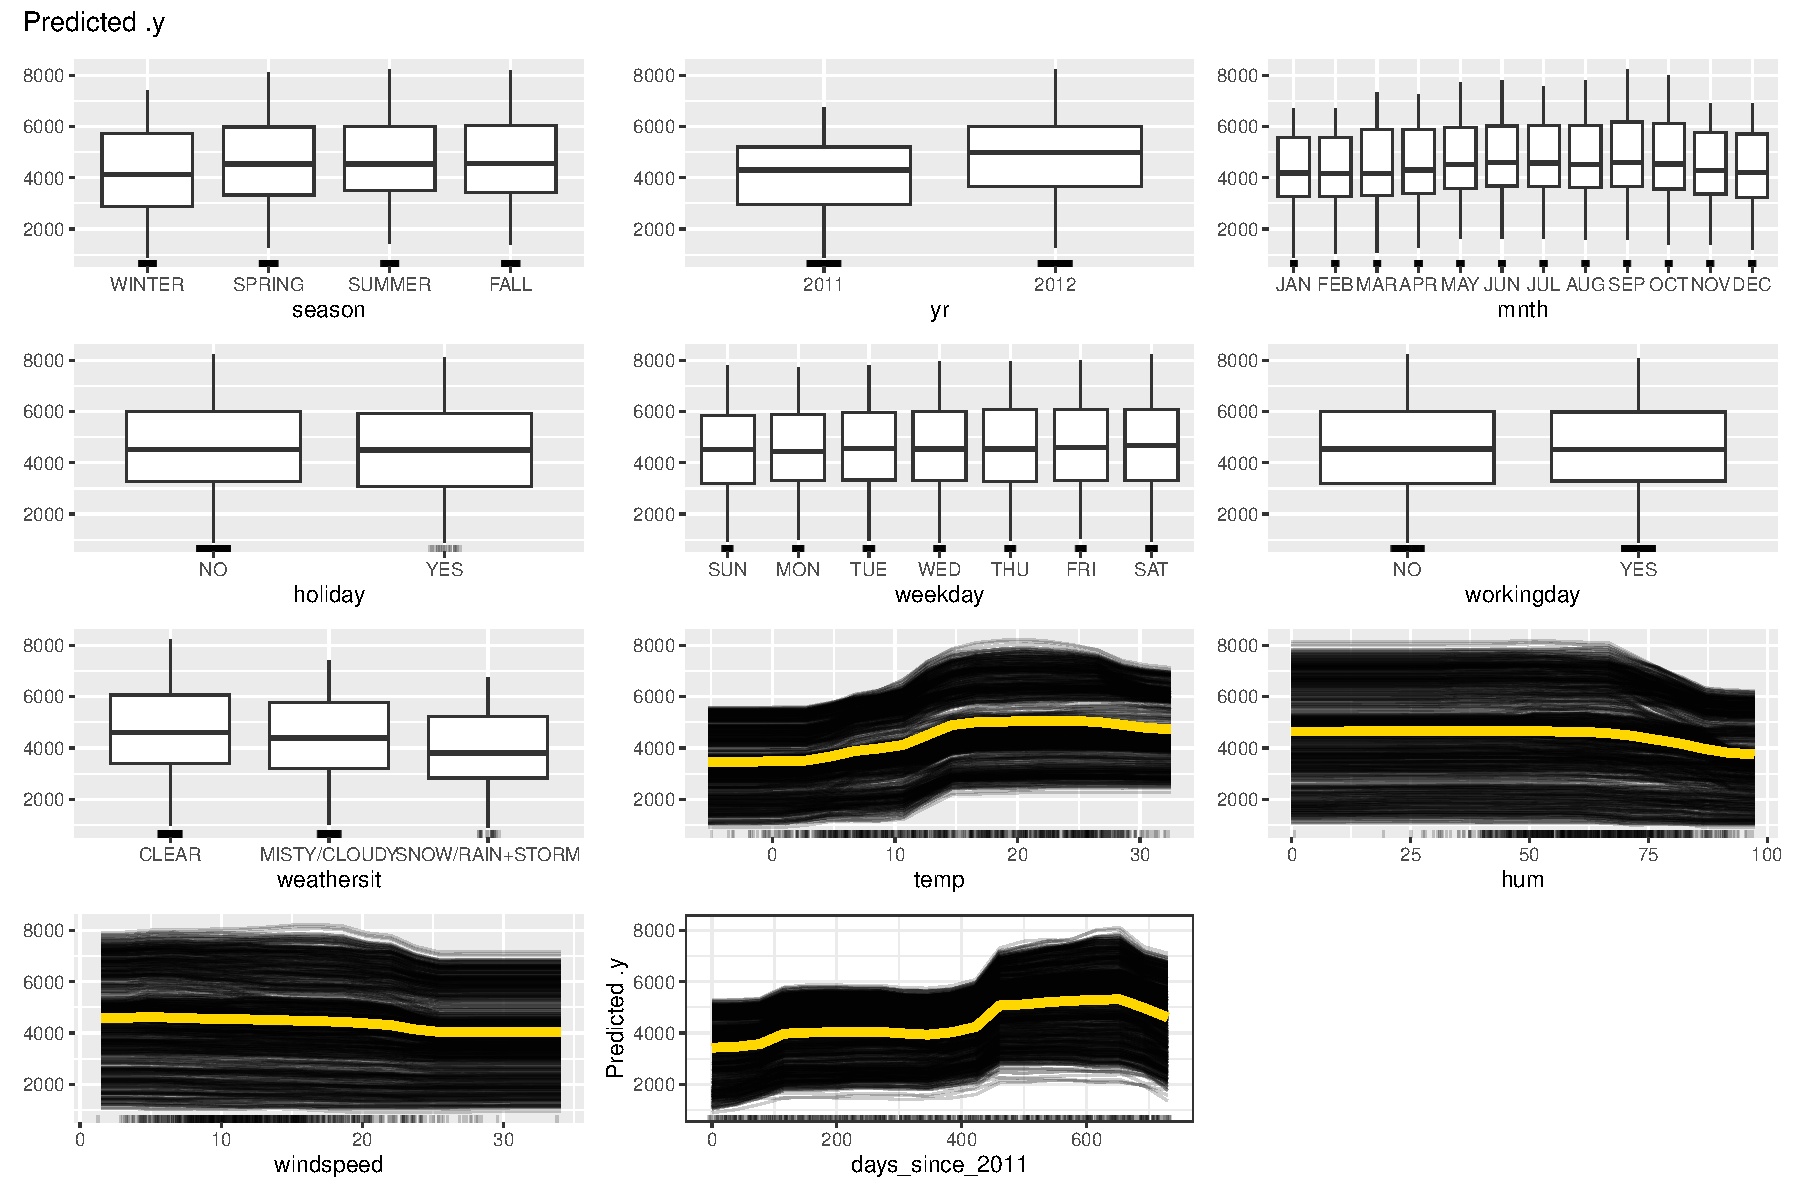
\includegraphics[width=0.6\linewidth]{figure_man/bike_pdp+ice} \hfill 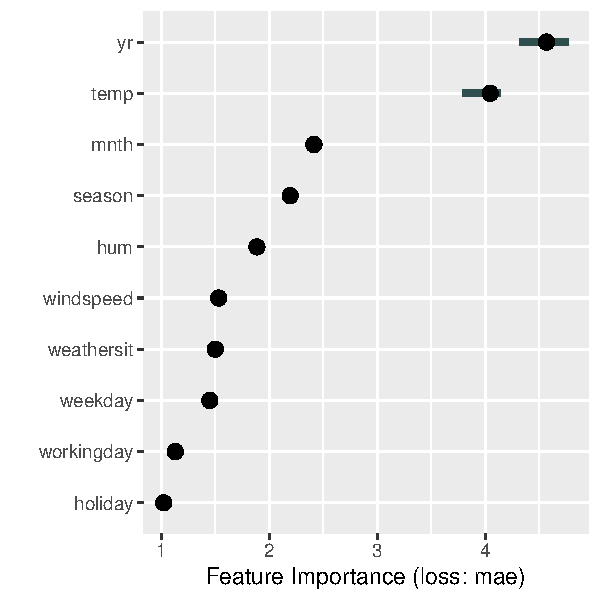
\includegraphics[width=0.35\linewidth]{figure_man/bike_pfi}
  \caption{A random forest was fit on the bike sharing dataset. Left: Partial dependence plots (PDP) for all features. Right: Feature importance plot (PFI).}
\end{figure}
\end{center}

\end{vbframe}

\begin{vbframe}{Feature Importance Scheme}
In general, feature importance methods share two components
\lz
\begin{enumerate}
  \item \textbf{Perturbation/Removal:} Generate predictions for which the feature of interest has been perturbed/removed.
  \item \textbf{Performance Comparison:} Compare performance under perturbation/removal with the original model performance.
\end{enumerate}
\lz
Depending on the type of perturbation/removal feature importance methods provide insight into different aspects of model and data.
\end{vbframe}


\begin{vbframe}{Potential Interpretation Goals}

Feature importance methods provide highly condensed insight, but can only highlight certain aspects of model and data. For example, one may be interested in getting insight into whether ...
\lz
\begin{enumerate}
    \item the feature $x_j$ is causal for the prediction?
    \begin{itemize}
      \item In a linear model: nonzero coefficient.
      \item More generally: changing the input to a feature $x_j$ has an effect on the prediction $\yh = \fh(x)$.
      \item \textit{Note:} A feature being causal for the prediction does not imply that the underlying variable is causal for the prediction target. For example, a disease symptom may be used to classify disease status (and is therefore causal for the prediction $\yh$). But intervening on the disease symptom does not have an effect on the disease and therefore is not causal for $y$.
    \end{itemize} \framebreak
    \item the variable $x_j$ contains prediction-relevant information?
    \begin{itemize}
      \item e.g. when $\E[y|x_j] \neq \E[y]$ for MSE loss
      \item More generally: The variable helps to predict the target quantity (e.g. conditional expectation), as measured by the difference in expected loss.
      \item If $x_j \indep y$ then $x_j$ and $y$ have zero mutual information and therefore cannot contain prediction-relevant information.
    \end{itemize}
    \item the model requires access to $x_j$ to achieve it's prediction performance?
    \begin{itemize}
      \item e.g. when $\E[y|x_{-j}] \neq \E[y|x_j, x_{-j}]$ for MSE loss
      \item More generally: The variable enables to improve the prediction of the target quantity over $x_{-j}$ only, as measured by the difference in expected loss.
      \item If $x_j \indep y | x_{-j}$ then $x_j$ cannot contain unique prediction-relevant information.
    \end{itemize}
\end{enumerate}
Except for special cases, these questions do not coincide.
\end{vbframe}

\begin{vbframe}{Potential Interpretation Goals}

The distinctness of the aforementioned aspects can be proven by example (sketch):

\begin{itemize}
  \item A feature may be causal for the prediction $\yh$ (1) without containing prediction-relevant information about $y$ (2). \textit{Example:} overfitting.
  \item A feature may contain prediction relevant information (2) without causing the prediction (1).  \textit{Examples:} underfitting, model multiplicity
  \item A feature may contain prediction-relevant information (2), without the model requiring access to the feature for (optimal) prediction performance (3).\\
  \textit{Note:} A model may rely on features that can be replace with others. E.g., a random forest model on dataset with $\E[y|x_1] \neq \E[y]$ and $\E[y|x_1] = \E[y|x_1, x_2]$ where $x_1$ was not sampled as potential split variable may rely on $x_2$.
  \end{itemize}
$\Rightarrow$ In general, an importance score cannot provide insight into all aspects at once.
\end{vbframe}

\begin{vbframe}
  %\textit{Note:} A model may rely on features that can be replace with others. E.g., a random forest model on dataset with $\E[y|x_1] \neq \E[y]$ and $\E[y|x_1] = \E[y|x_1, x_2]$ where $x_1$ was not sampled as potential split variable may rely on $x_2$. 
  \begin{figure}
  \begin{tikzpicture}[thick, scale=1.25, every node/.style={scale=1, line width=0.25mm, black, fill=white}]
		%
		\node[draw, ellipse, scale=0.7] (x0) at (0, 2) {trust};
		\node[draw, ellipse, scale=0.7] (x1) at (0, 1) {vaccinated};
		\node[draw, ellipse, scale=0.7] (x2) at (0, 0) {contact};
		\node[draw, ellipse, scale=0.7] (x3) at (0,-1) {cough};
		\node[draw, ellipse, scale=0.7] (x4) at (0,-2) {test};
		\node[draw, ellipse, scale=0.7] (x5) at (0,-3) {compliance};
		\node[draw, ellipse, scale=0.7] (y) at (-2,-.5) {$Y$: CoViD risk};
		\draw[dashed,gray] (-3,-3.5) -- (.75,-3.5) -- (.75,2.5) -- (-3,2.5) -- cycle;
		\node[scale=0.7] (dots) at (-1,-3.75) {data level, variables};
		\draw[->] (x0) -- (x1);
		\draw[->] (x1) -- (y);
		\draw[->] (x2) -- (y);
		\draw[->] (y) -- (x3);
		\draw[->] (y) -- (x4);
		\draw[->] (x5) -- (x4);
		%\draw[-] (xd) -- (y);
		
		\node[draw, ellipse, scale=0.7] (ux0) at (2, 2) {\texttt{trust}};
		\node[draw, ellipse, scale=0.7] (ux1) at (2, 1) {\texttt{vac}};
		\node[draw, ellipse, scale=0.7] (ux2) at (2, 0) {\texttt{con}};
		\node[draw, ellipse, scale=0.7] (ux3) at (2,-1) {\texttt{cough}};
		\node[draw, ellipse, scale=0.7] (ux4) at (2,-2) {\texttt{test}};
		\node[draw, ellipse, scale=0.7] (ux5) at (2,-3) {\texttt{cmpl}};

		\draw[dashed,gray] (1.25,-3.5) -- (3.5,-3.5) -- (3.5,2.5) -- (1.25,2.5) -- cycle;
		\node[scale=0.7] (dots) at (2.5,-3.75) {model level, features};
		\draw[->, dotted] (x1) -- (ux1);
		\draw[->, dotted] (x2) -- (ux2);
		\draw[->, dotted] (x3) -- (ux3);
		\draw[->, dotted] (x4) -- (ux4);
		\draw[->, dotted] (x0) -- (ux0);
		\draw[->, dotted] (x5) -- (ux5);
		
		\node[draw, circle, scale=0.7] (yhat) at (3, -.5) {$\hat{Y}$};
		\draw[->] (ux1) -- (yhat);
		\draw[->] (ux2) -- (yhat);
		\draw[->] (ux3) -- (yhat);
		\draw[->] (ux4) -- (yhat);
		\draw[->] (ux5) -- (yhat);
\end{tikzpicture}
\end{figure} 
\end{vbframe}


\endlecture
\end{document}
